\begin{appendices}

\section{Impact du chlore} 
\label{appendix:chlore}

\begin{figure}[!htbp]
    \centering
    \begin{subfigure}[t]{0.49\textwidth} % "0.49" donne ici la largeur de l'image
        \centering 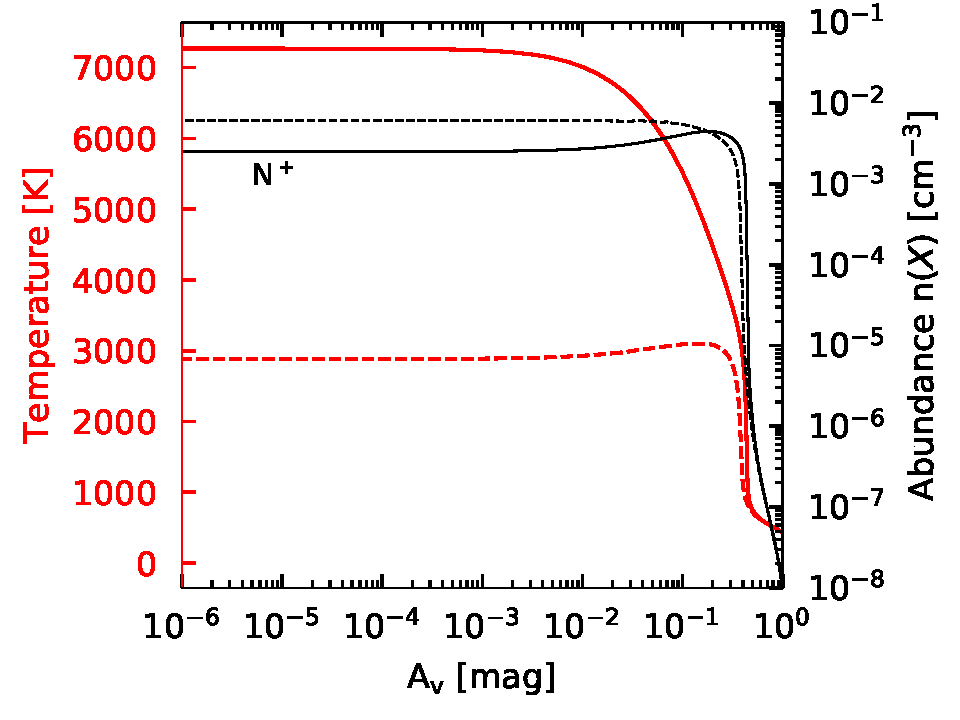
\includegraphics[trim = {0 0 0 0},clip,width=1\textwidth]{figure/Cl/gridModelEmiss/nT_comp_Np.pdf}
        \caption{$\mathrm{N}^+$}
    \end{subfigure}
    ~ 
   \begin{subfigure}[t]{0.49\textwidth} % "0.49" donne ici la largeur de l'image
        \centering 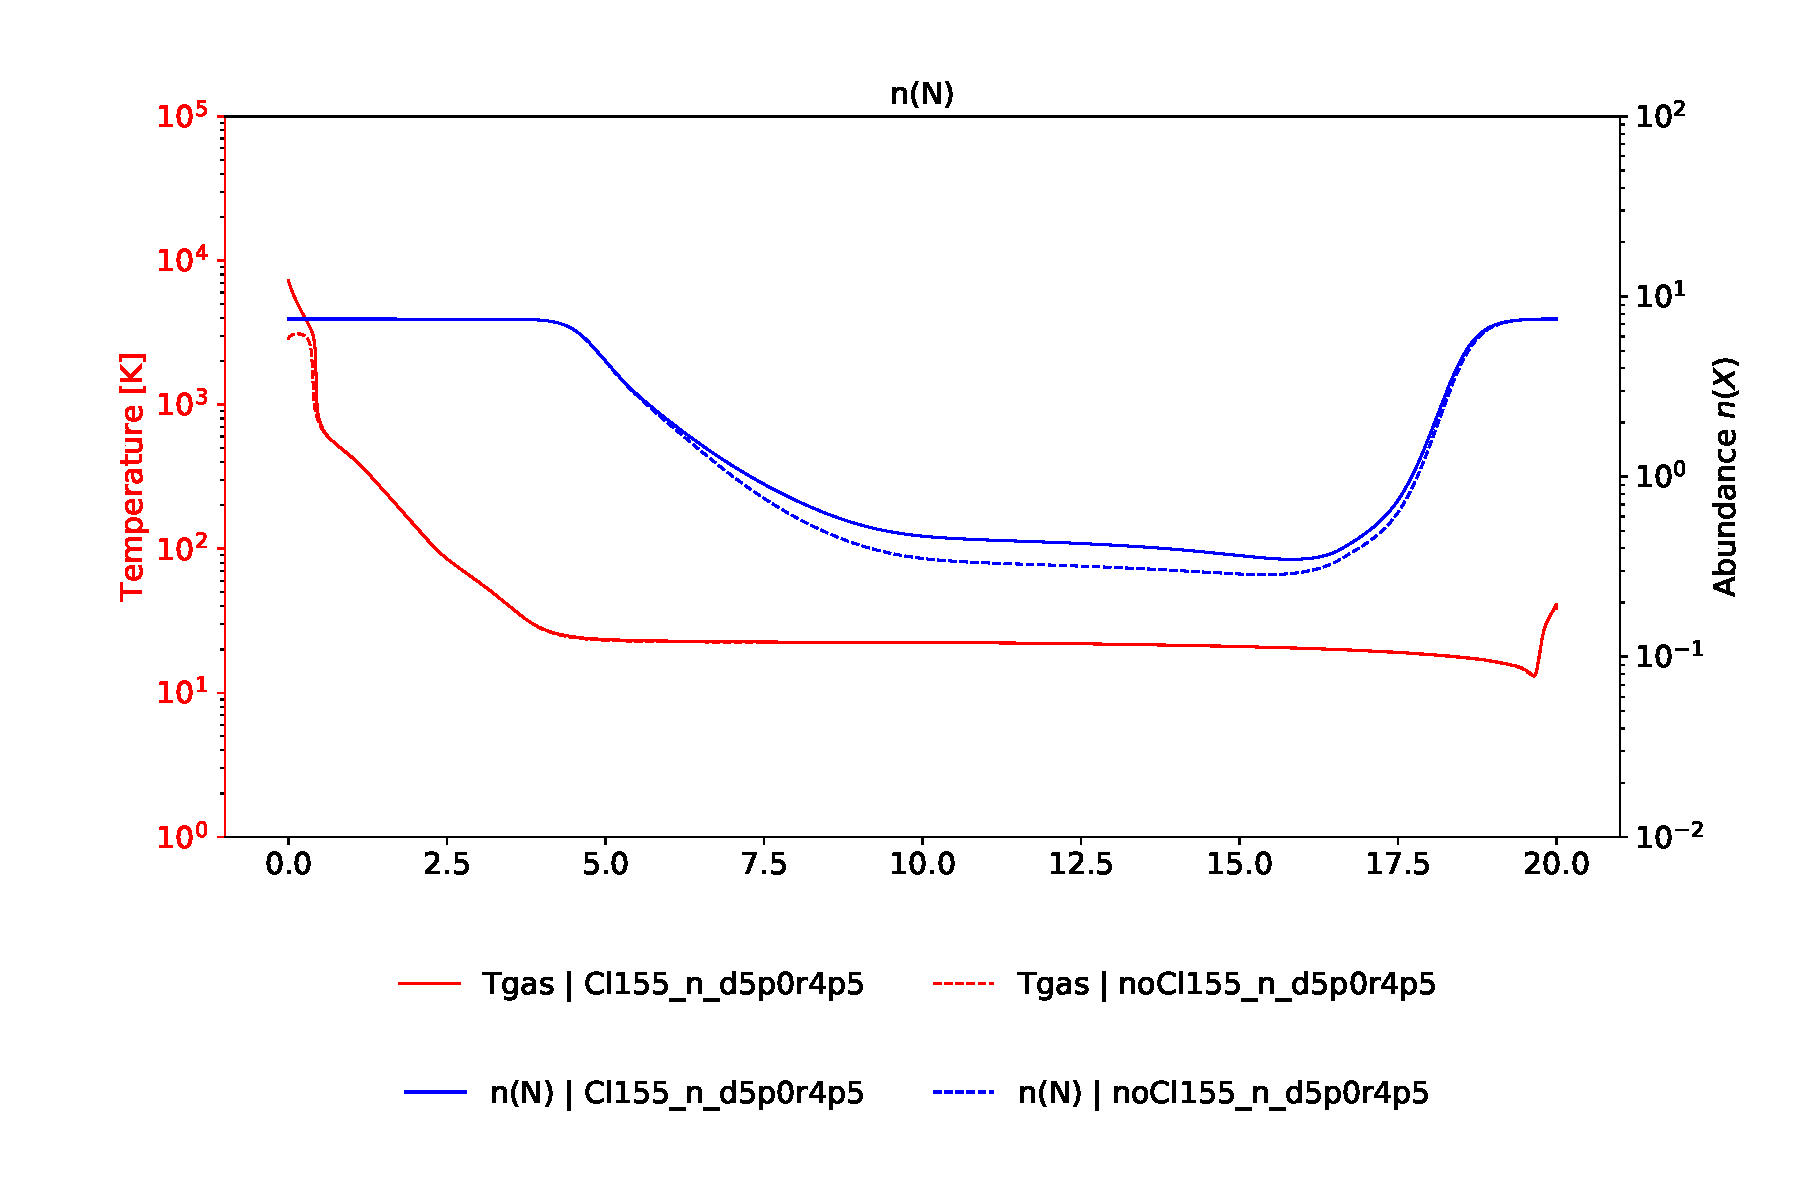
\includegraphics[trim = {0 0 0 0},clip,width=1\textwidth]{figure/Cl/gridModelEmiss/nT_comp_N.pdf}
        \caption{$\mathrm{N}$}
    \end{subfigure}
    
    \begin{subfigure}[t]{0.49\textwidth} % "0.49" donne ici la largeur de l'image
        \centering 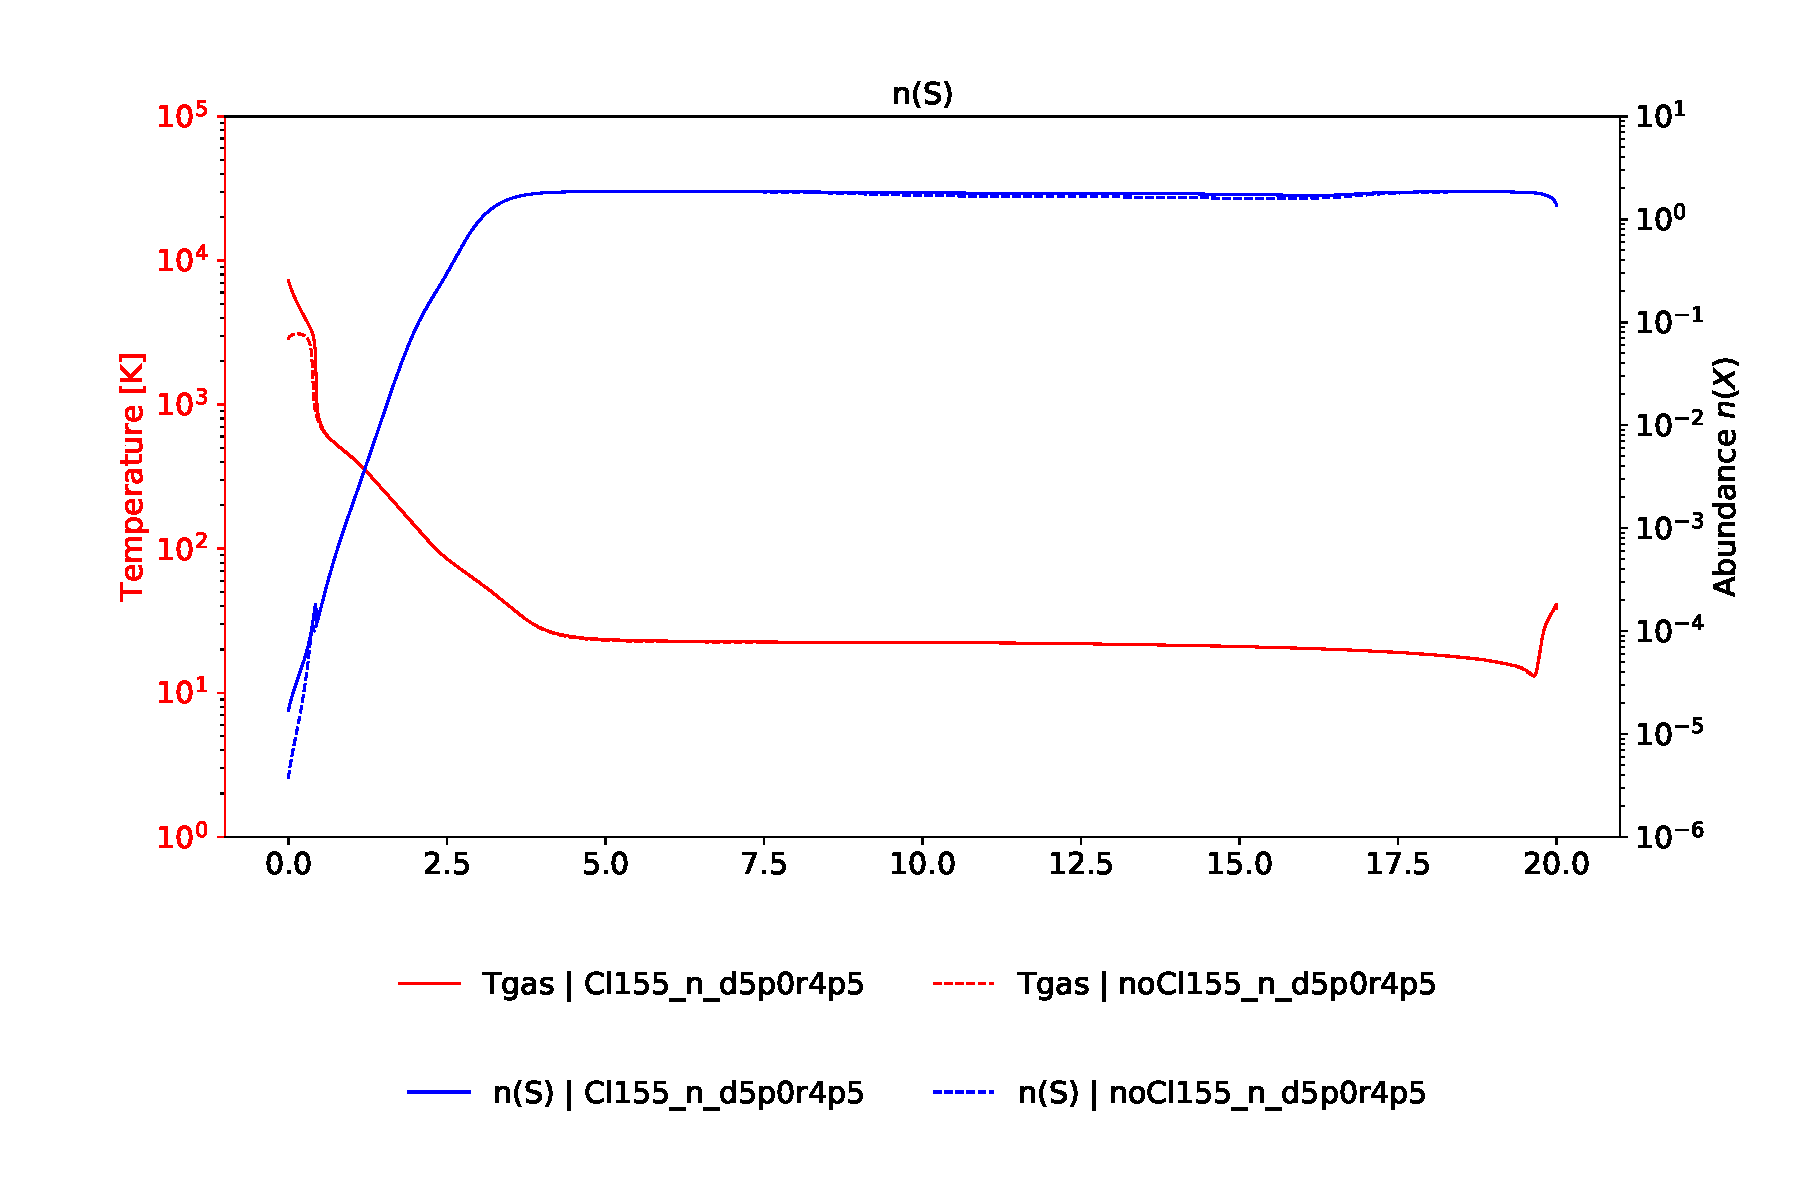
\includegraphics[trim = {0 0 0 0},clip,width=1\textwidth]{figure/Cl/gridModelEmiss/nT_comp_S.pdf}
        \caption{$\mathrm{S}$}
    \end{subfigure}
    ~
    \begin{subfigure}[t]{0.49\textwidth} % "0.49" donne ici la largeur de l'image
        \centering 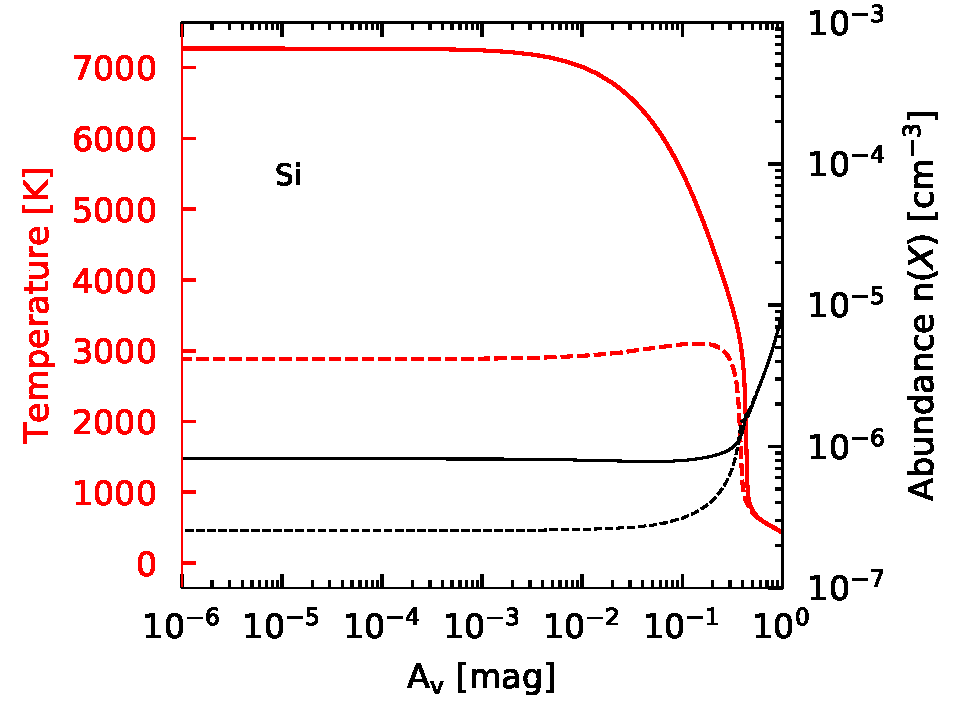
\includegraphics[trim = {0 0 0 0},clip,width=1\textwidth]{figure/Cl/gridModelEmiss/nT_comp_Si.pdf}
        \caption{$\mathrm{Si}$}
    \end{subfigure}
    
    \caption{(ANNEXE) Profils de densité des traceurs impactés par l'ajout du chlore.}
    \begin{minipage}{\textwidth}
    Il est représenté en trait plein les profils du modèle avec le chlore et en trait pointillé le modèle ne contenant pas de chlore. La température est en rouge et la densité en noir.
    \end{minipage}
    \label{fig:Cl:gridModelEmiss:nT:yes}
\end{figure}

\begin{figure}[!htbp]
    \centering
    \begin{subfigure}[t]{0.49\textwidth} % "0.49" donne ici la largeur de l'image
        \centering 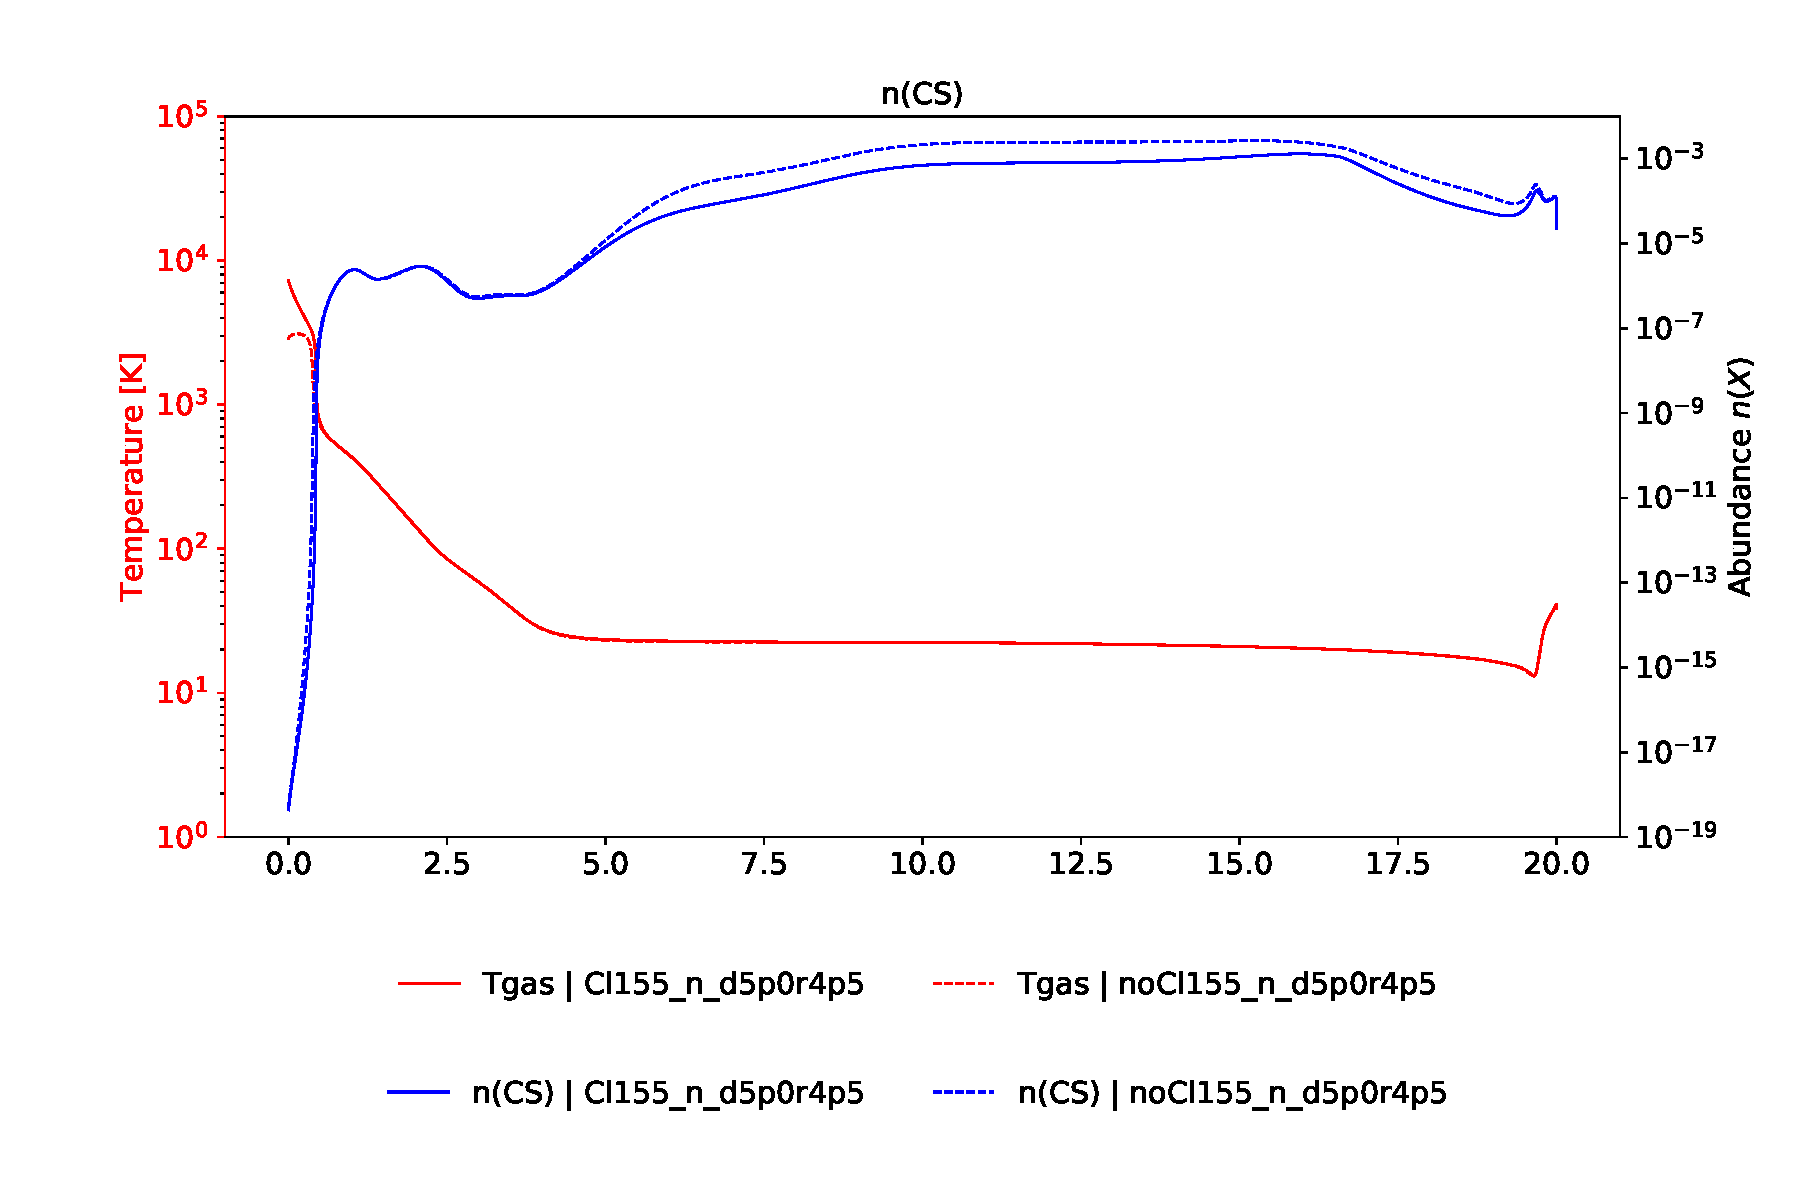
\includegraphics[trim = {0 0 0 0},clip,width=1\textwidth]{figure/Cl/gridModelEmiss/nT_comp_CS.pdf}
        \caption{$\mathrm{CS}$}
    \end{subfigure}
    ~ 
   \begin{subfigure}[t]{0.49\textwidth} % "0.49" donne ici la largeur de l'image
        \centering 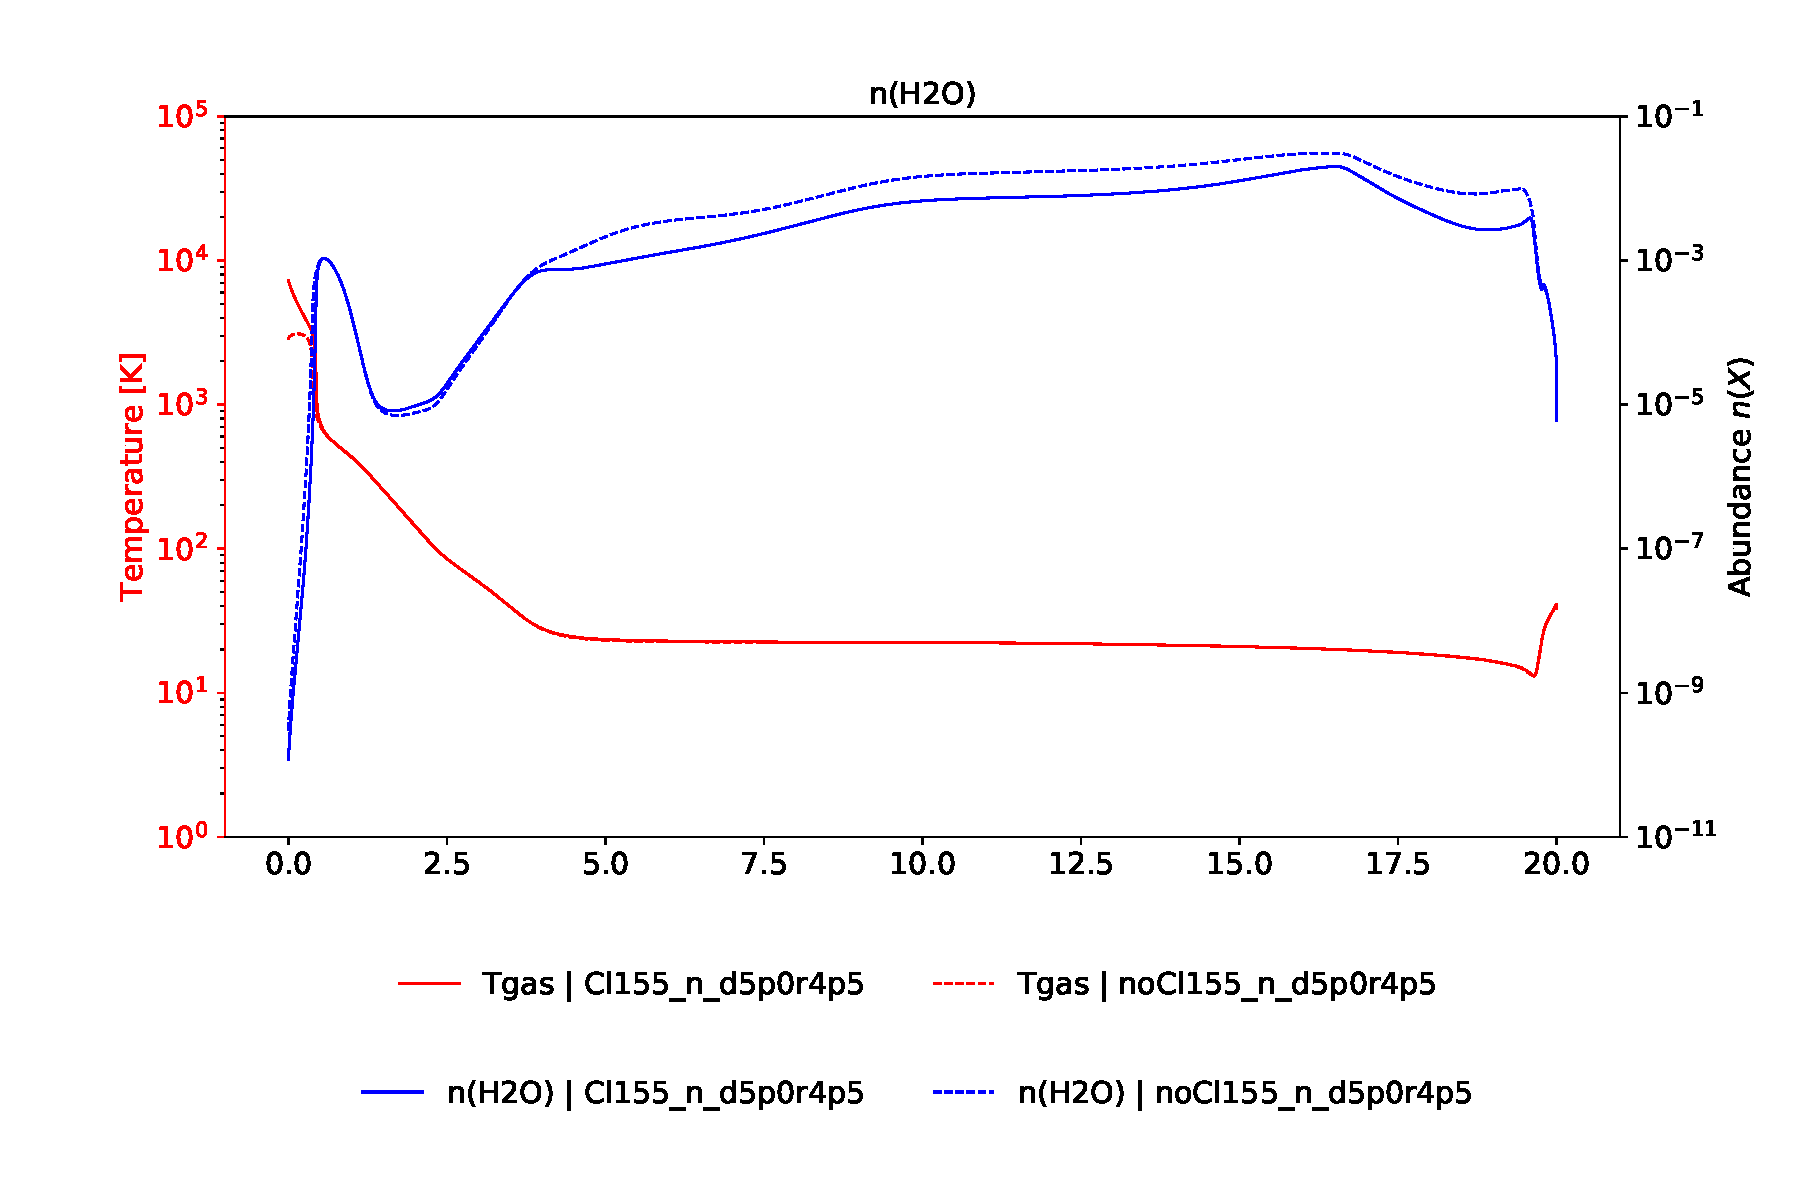
\includegraphics[trim = {0 0 0 0},clip,width=1\textwidth]{figure/Cl/gridModelEmiss/nT_comp_H2O.pdf}
        \caption{$\mathrm{H}_2\mathrm{O}$}
    \end{subfigure}
    
    \begin{subfigure}[t]{0.49\textwidth} % "0.49" donne ici la largeur de l'image
        \centering 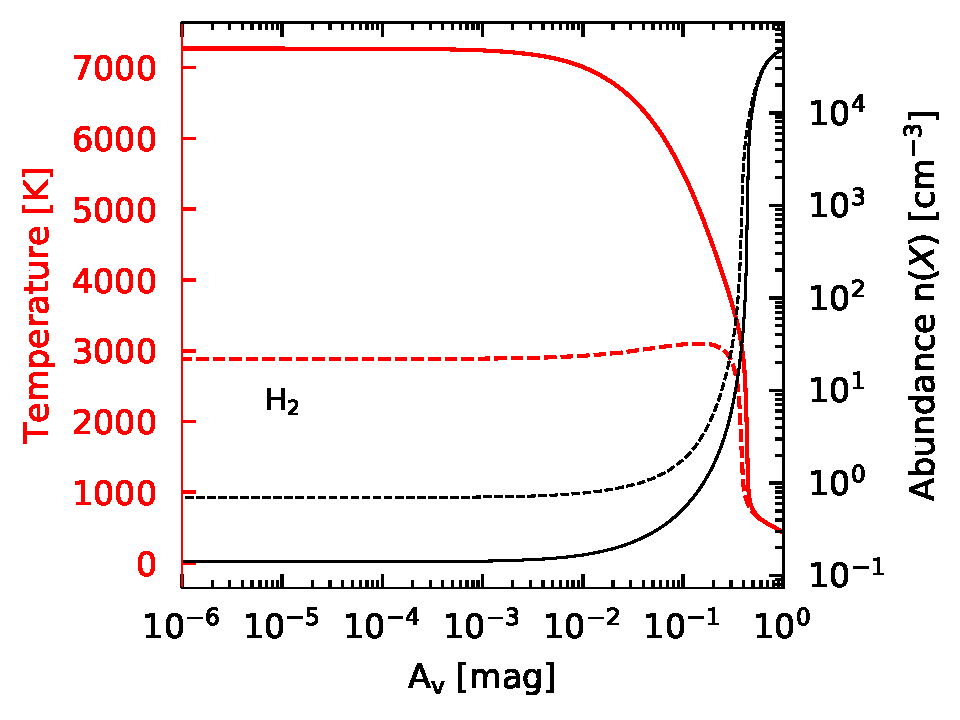
\includegraphics[trim = {0 0 0 0},clip,width=1\textwidth]{figure/Cl/gridModelEmiss/nT_comp_H2.pdf}
        \caption{$\mathrm{H}_2$}
    \end{subfigure}
    ~ 
    \begin{subfigure}[t]{0.49\textwidth} % "0.49" donne ici la largeur de l'image
        \centering 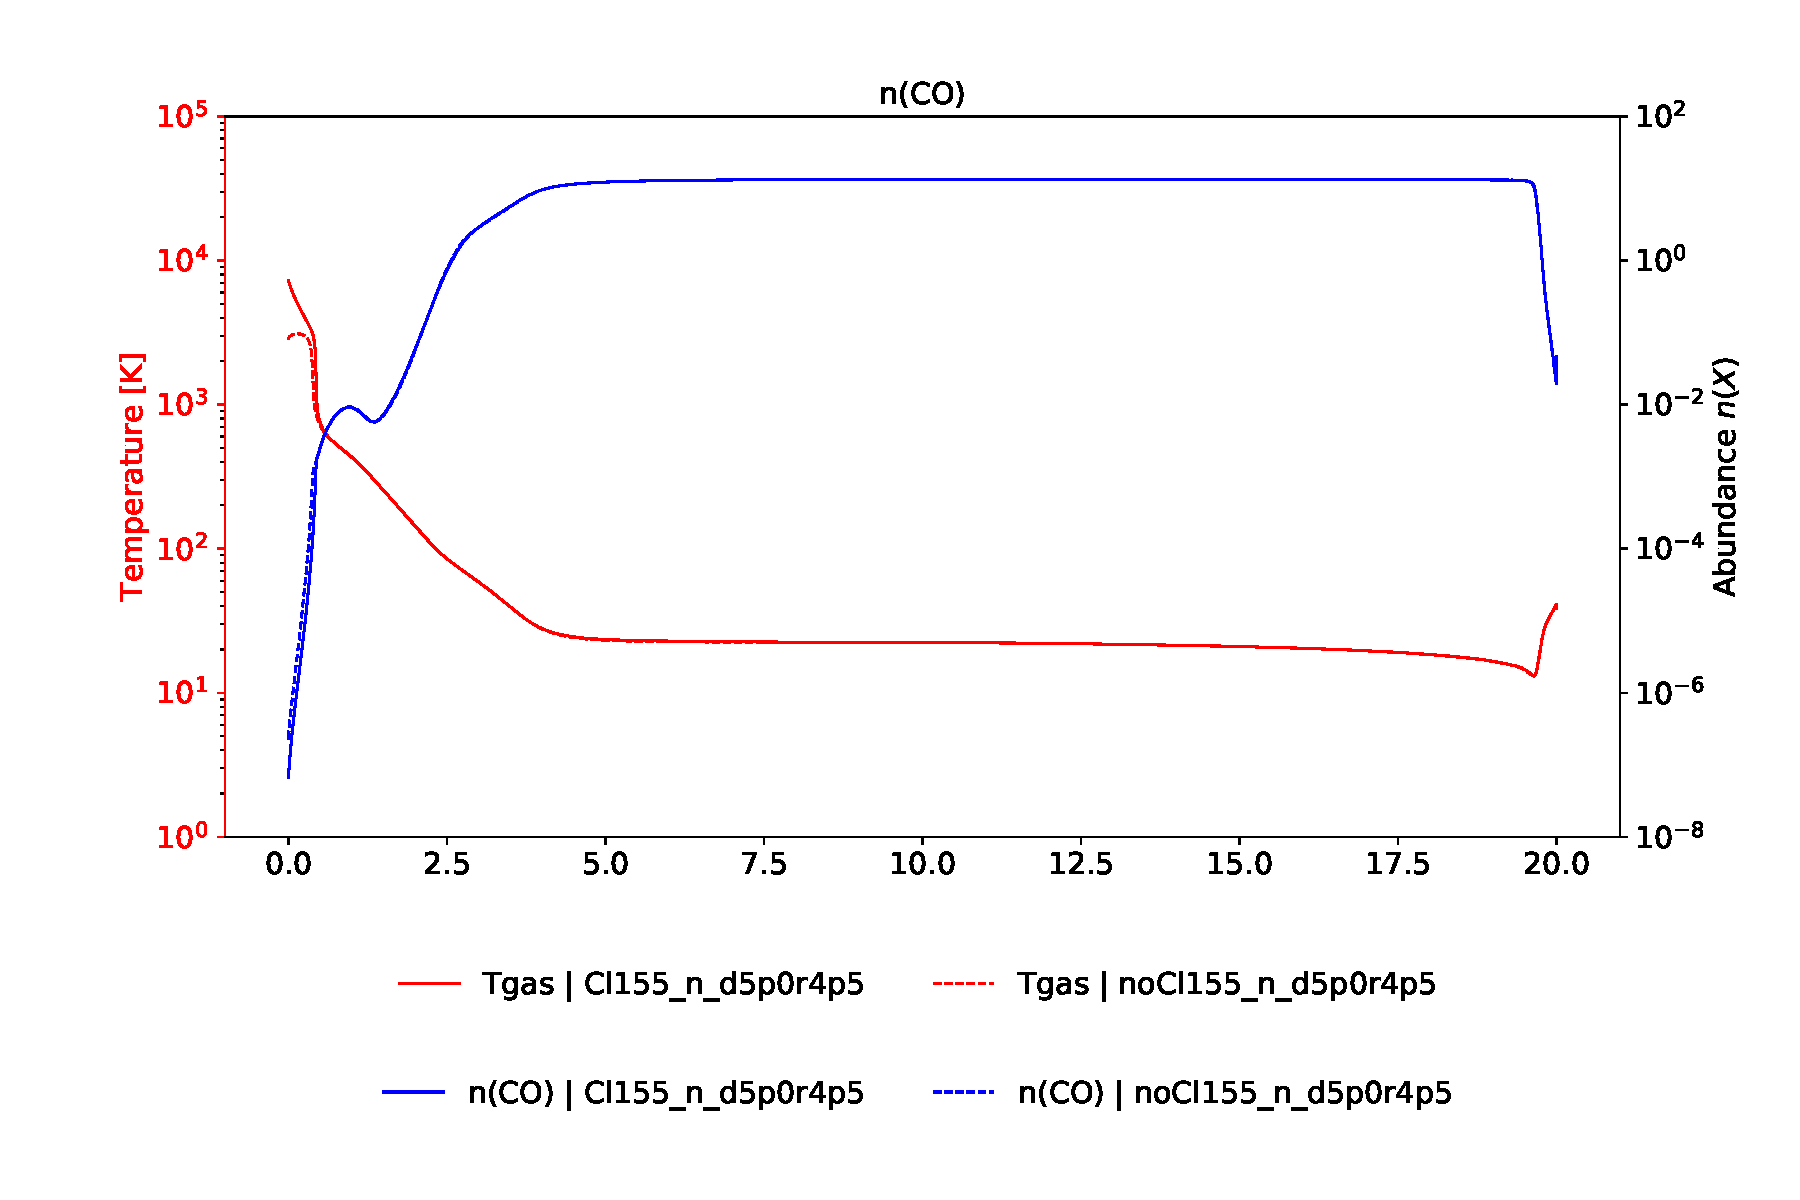
\includegraphics[trim = {0 0 0 0},clip,width=1\textwidth]{figure/Cl/gridModelEmiss/nT_comp_CO.pdf}
        \caption{$\mathrm{CO}$}
    \end{subfigure}
    
    \caption{((ANNEXE) Profils de densité des traceurs impactés par l'ajout du chlore. Mêmes conventions que pour la figure \ref{fig:Cl:gridModelEmiss:nT:yes}.}
    \label{fig:Cl:gridModelEmiss:nT:no}
\end{figure}


\begin{figure}[!h]
    \centering
    \begin{subfigure}[t]{0.49\textwidth} % "0.49" donne ici la largeur de l'image
        \centering 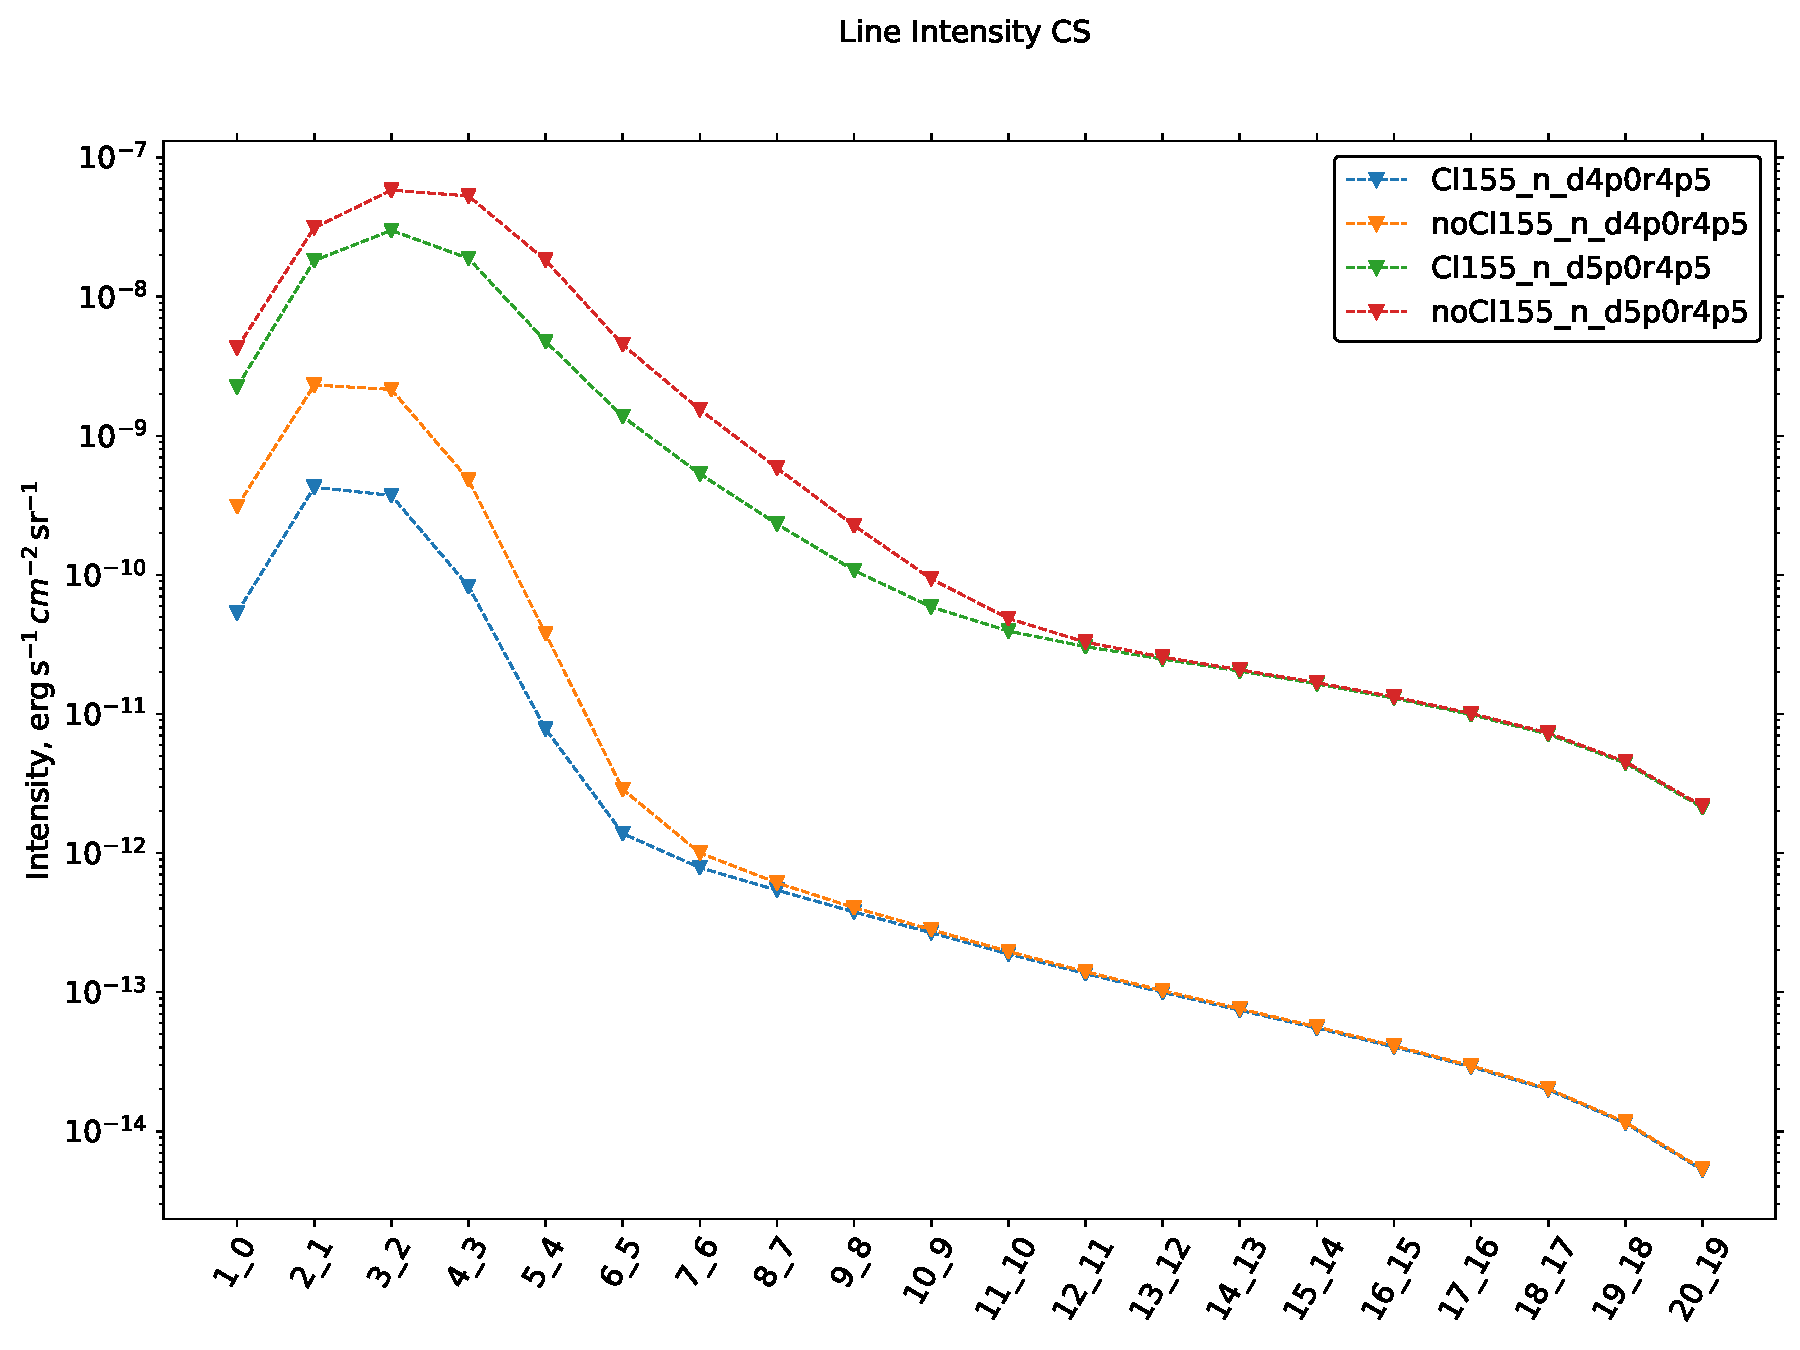
\includegraphics[trim = {0 0 0 1cm},clip,width=1\textwidth]{figure/Cl/gridModelEmiss/I_comp_CS.pdf}
        \caption{$\mathrm{CS}$}
    \end{subfigure}
    ~ 
   \begin{subfigure}[t]{0.49\textwidth} % "0.49" donne ici la largeur de l'image
        \centering 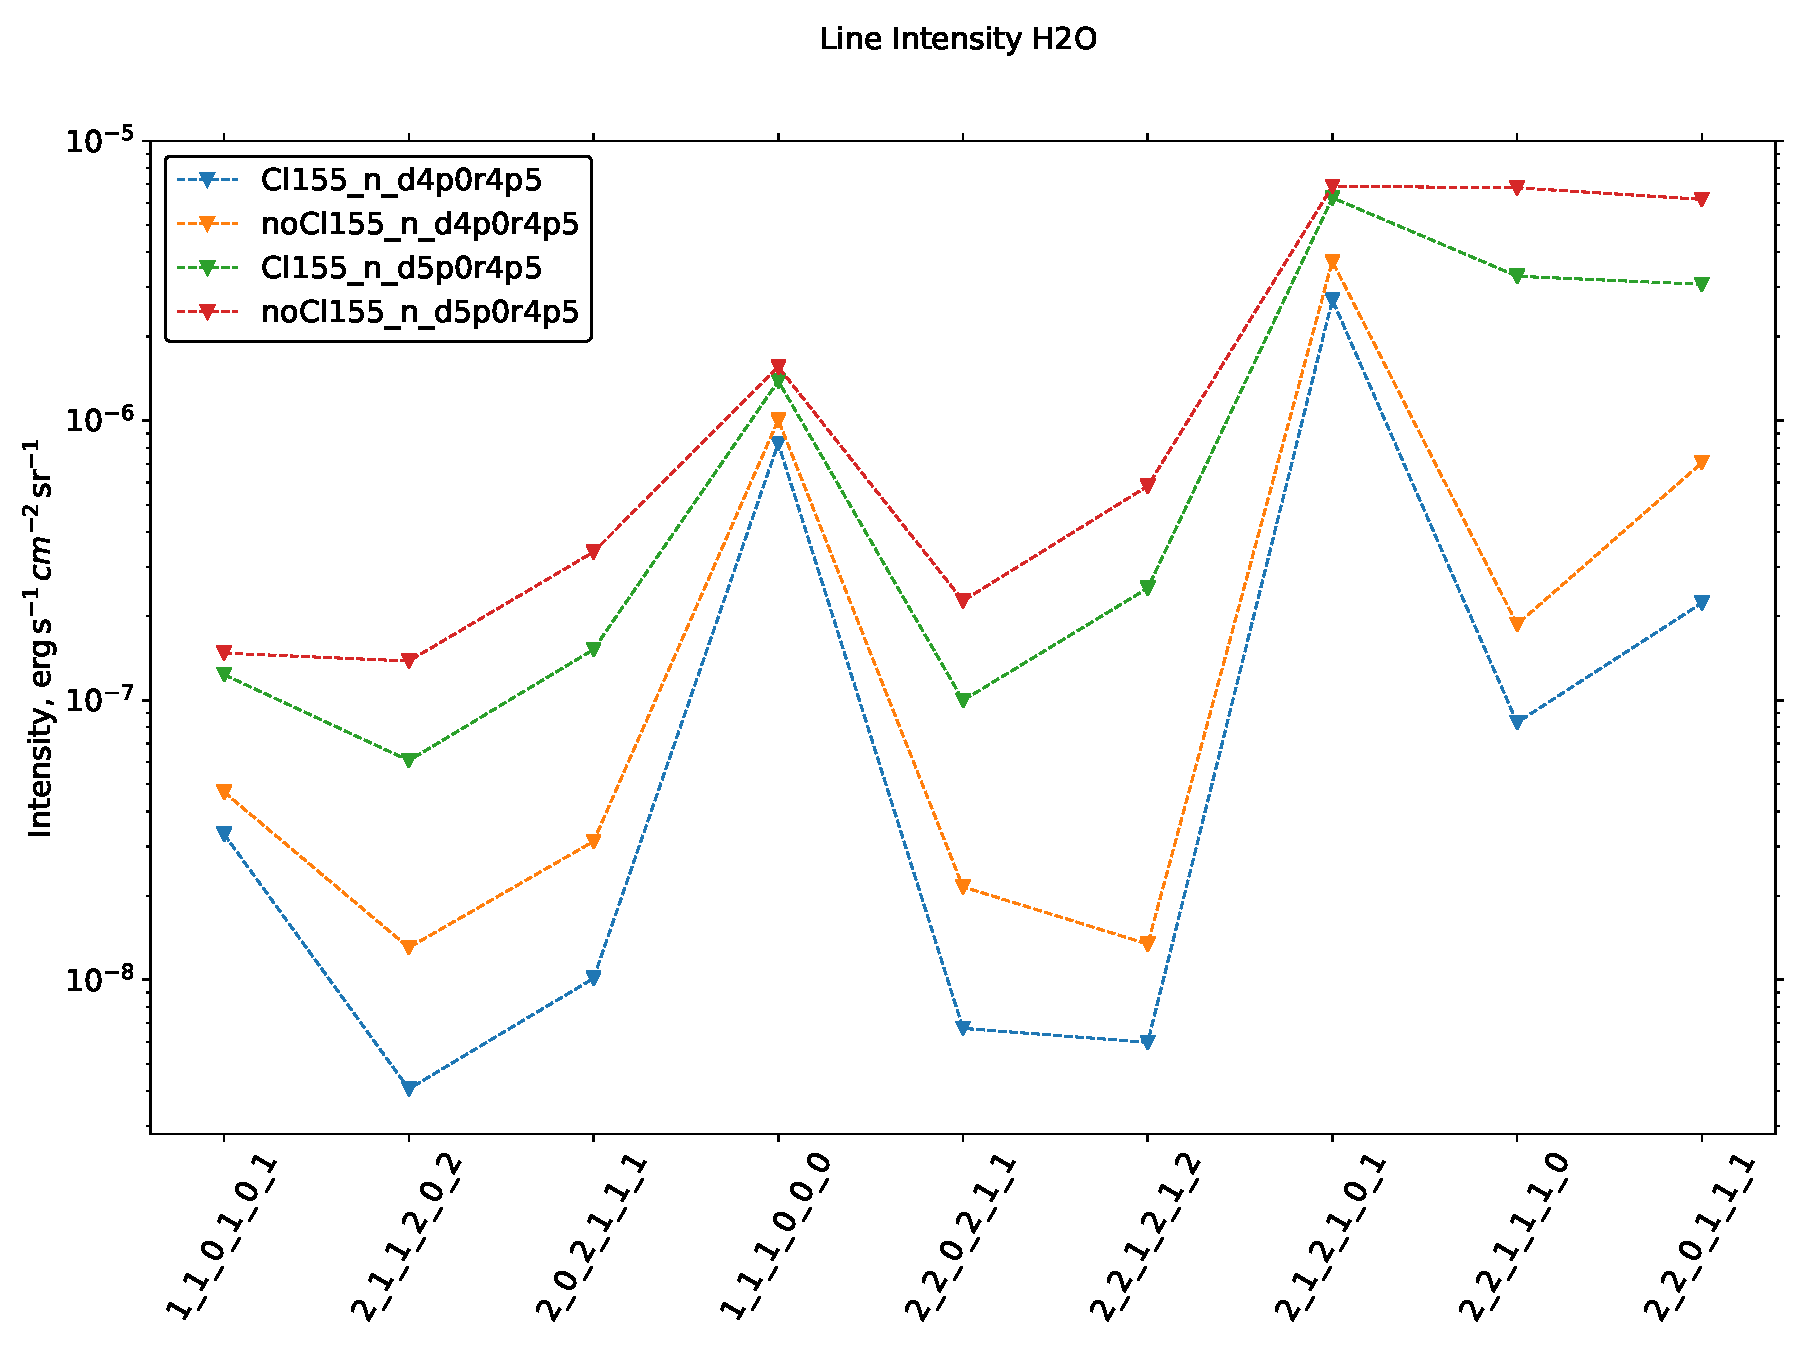
\includegraphics[trim = {0 0 0 1cm},clip,width=1\textwidth]{figure/Cl/gridModelEmiss/I_comp_H2O.pdf}
        \caption{$\mathrm{H}_2\mathrm{O}$}
    \end{subfigure}
    
    \begin{subfigure}[t]{0.49\textwidth} % "0.49" donne ici la largeur de l'image
        \centering 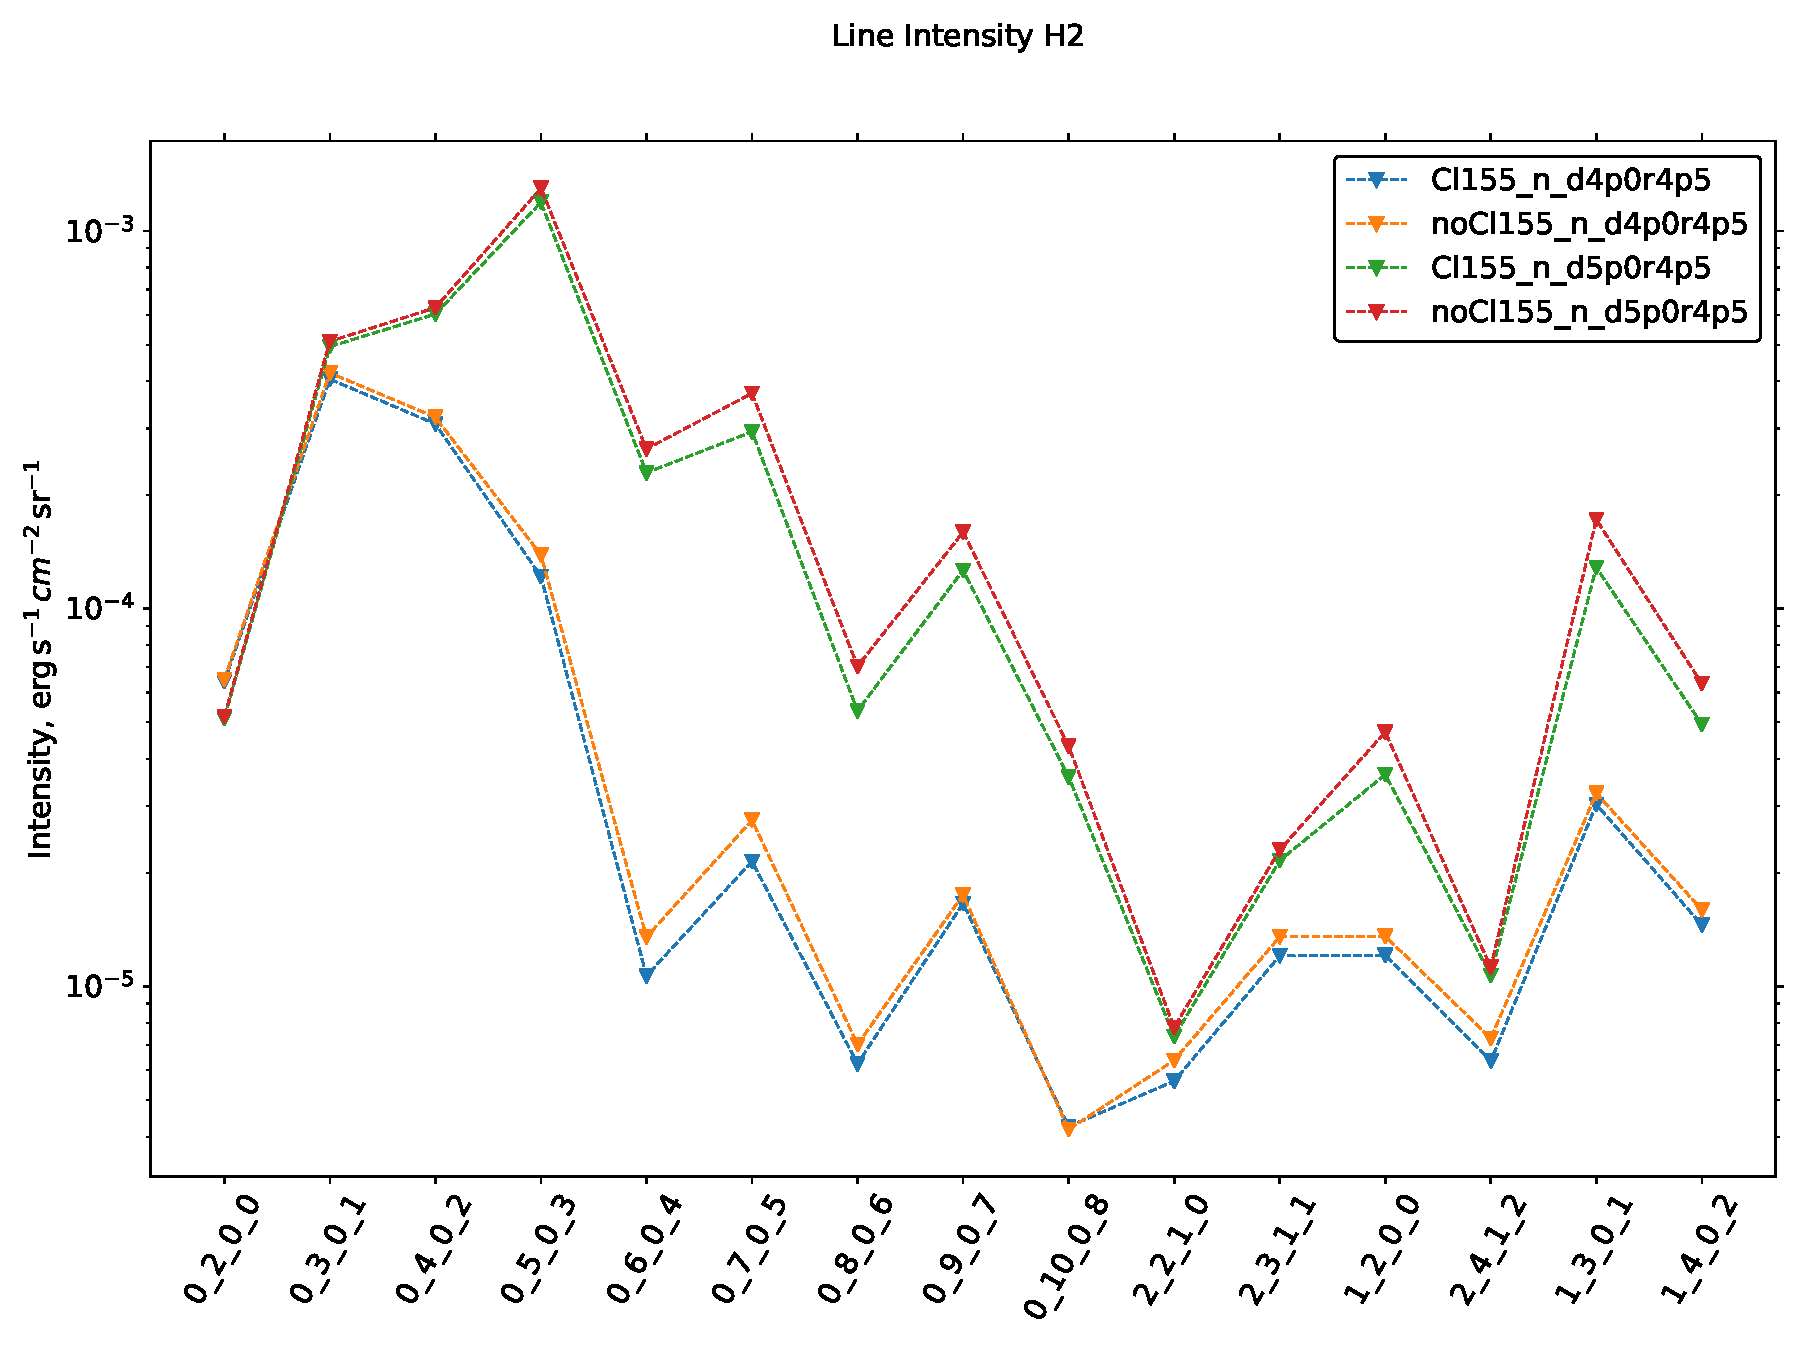
\includegraphics[trim = {0 0 0 1cm},clip,width=1\textwidth]{figure/Cl/gridModelEmiss/I_comp_H2.pdf}
        \caption{$\mathrm{H}_2$}
    \end{subfigure}
    ~ 
    \begin{subfigure}[t]{0.49\textwidth} % "0.49" donne ici la largeur de l'image
        \centering 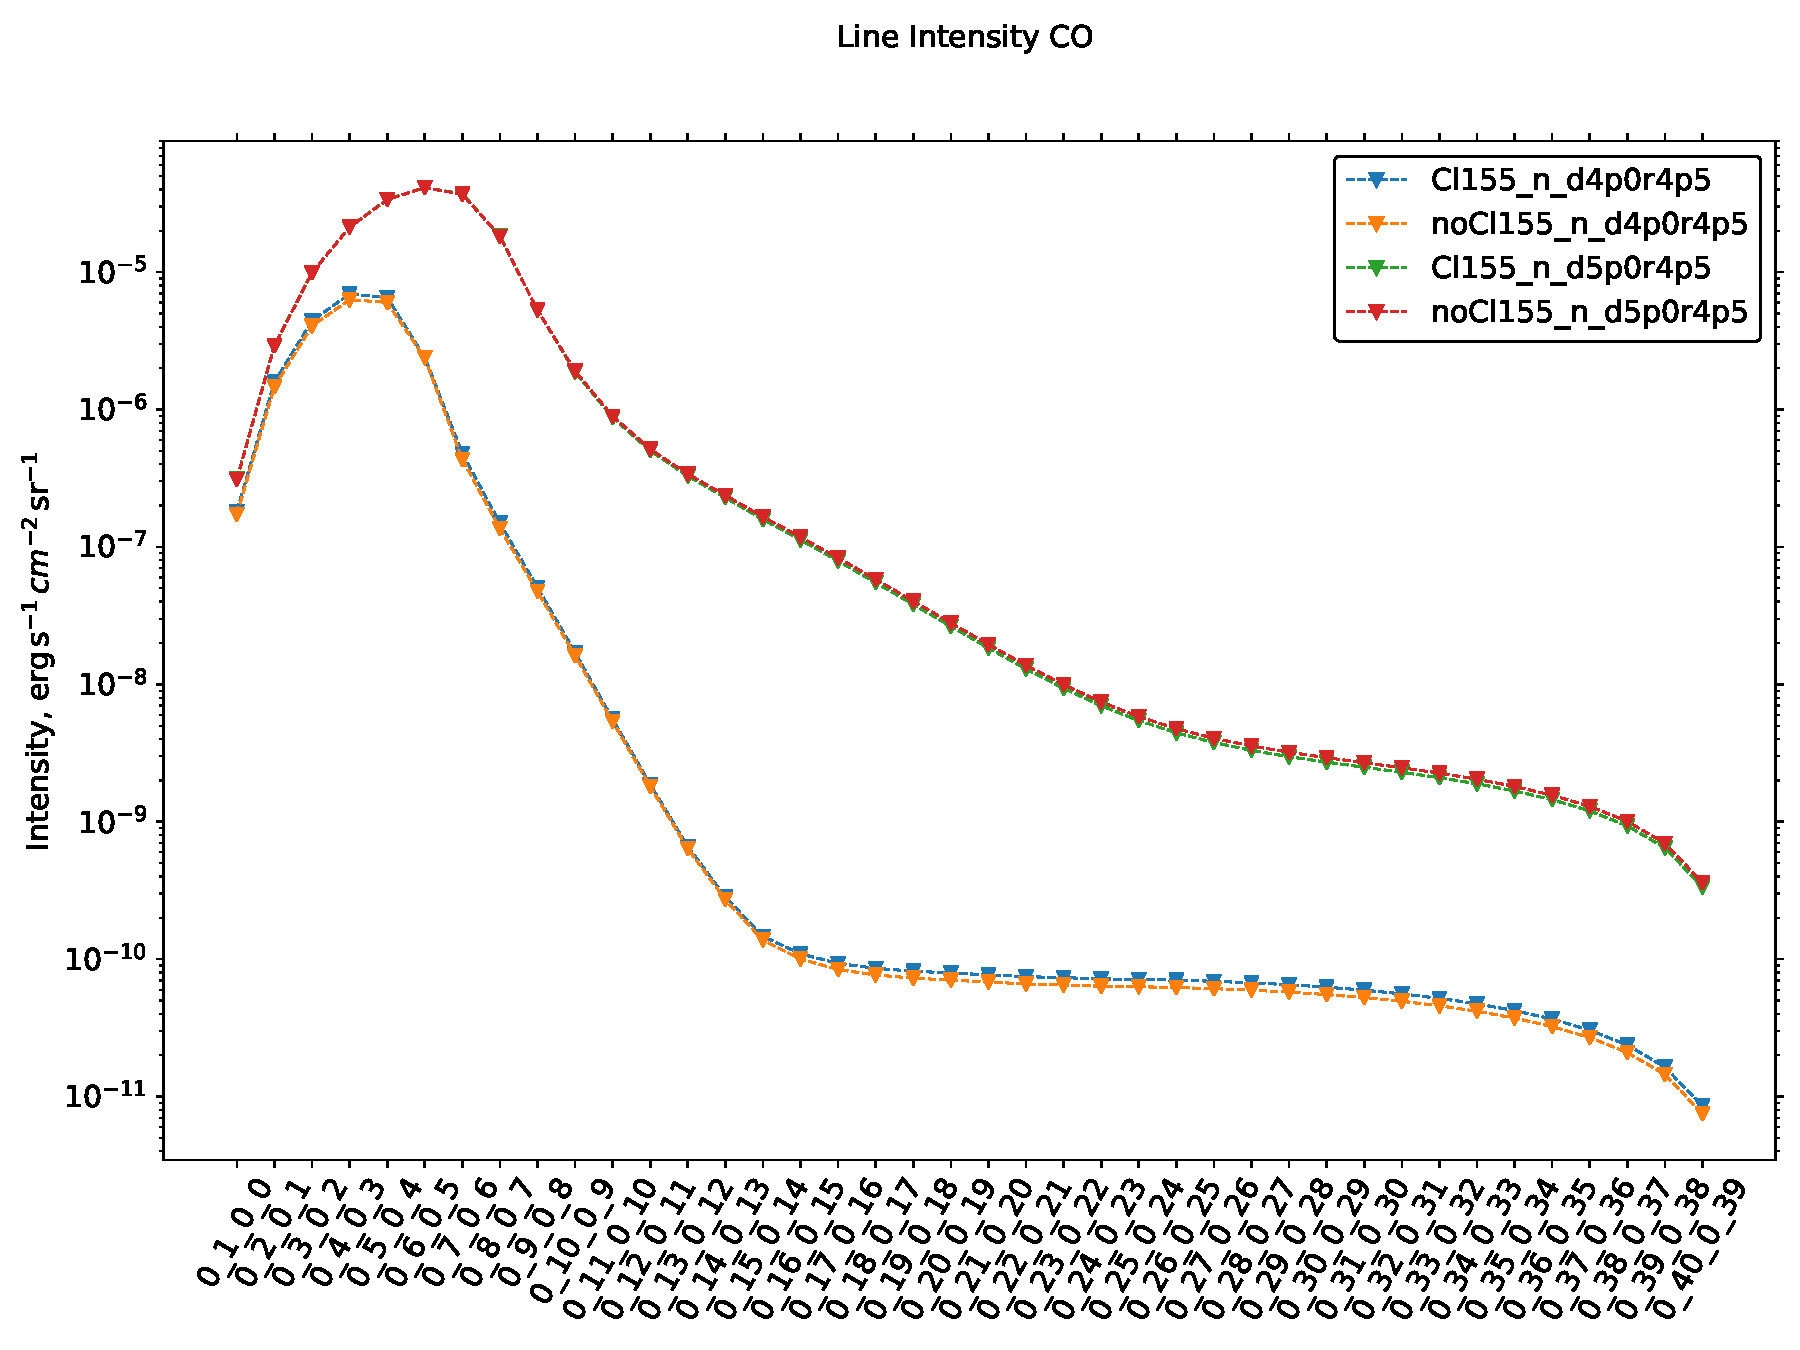
\includegraphics[trim = {0 0 0 1cm},clip,width=1\textwidth]{figure/Cl/gridModelEmiss/I_comp_CO.pdf}
        \caption{$\mathrm{CO}$}
    \end{subfigure}
    
    \caption{(ANNEXE) Diagramme d'excitation des traceurs peu modifiés par l'ajout du chlore dans le code PDR (même convention que la figure \ref{fig:Cl:gridModelEmiss:yes}). Pour la molécule $\mathrm{CO}$, les transitions rotationnelles ont été écrites (toutes s'effectuent à $\mathrm{v}=0$).}
    \label{fig:Cl:gridModelEmiss:no}
\end{figure}


%%%%%%%%%%%%%%%%%%%%%%%%%%%%%%%%%%%%%%%%%%%%%%%%%%%%%%%%%%%%%%%%%%%%%%%%%%%%%%%%%%%%%%%%%%%%%
\clearpage
\section{$\mathrm{H}_2$ excité}
\label{appendix:type46}
\begin{figure}[!h]
    \centering 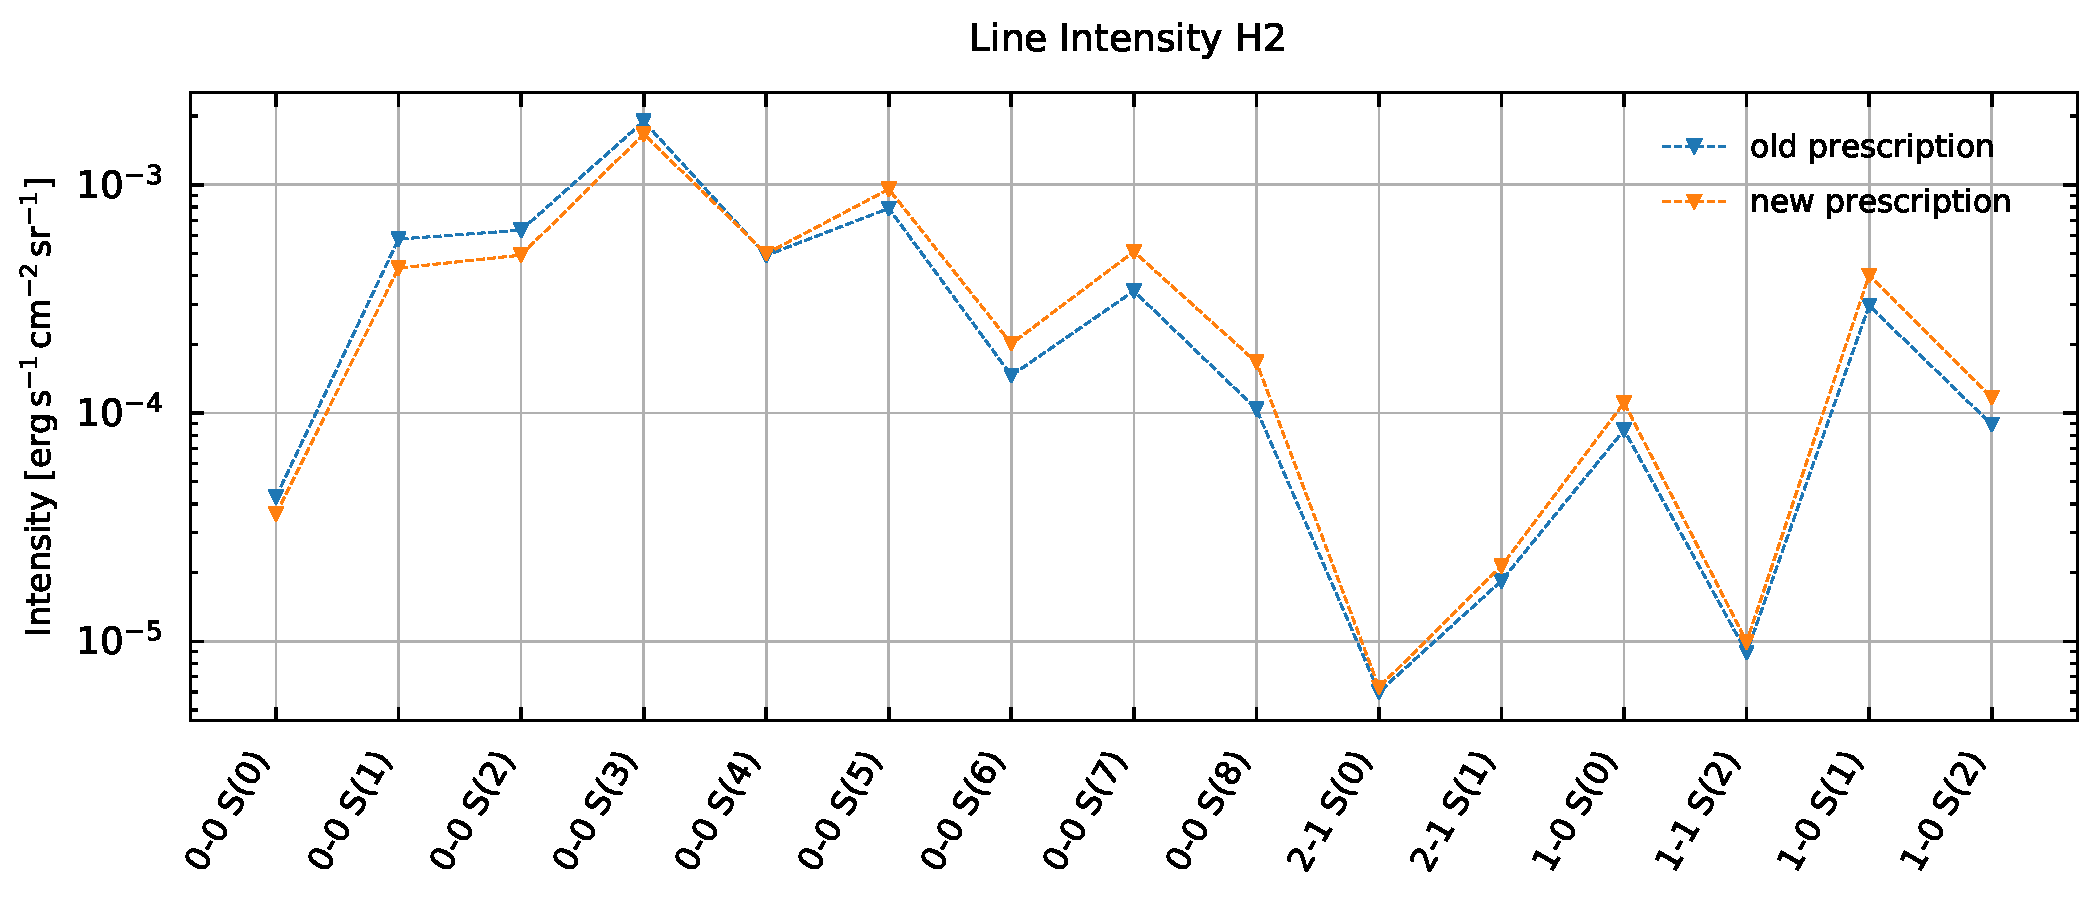
\includegraphics[trim = {0 0 0 1cm},clip,width=0.8\textwidth]{figure/type46/I_comp_H2.pdf}
    \caption{Diagramme d'excitation du $\mathrm{H}_2$}
    \begin{minipage}{\textwidth}
    
    \end{minipage}
    \label{fig:type46:H2}
\end{figure}

\begin{figure}[!h]
    \centering 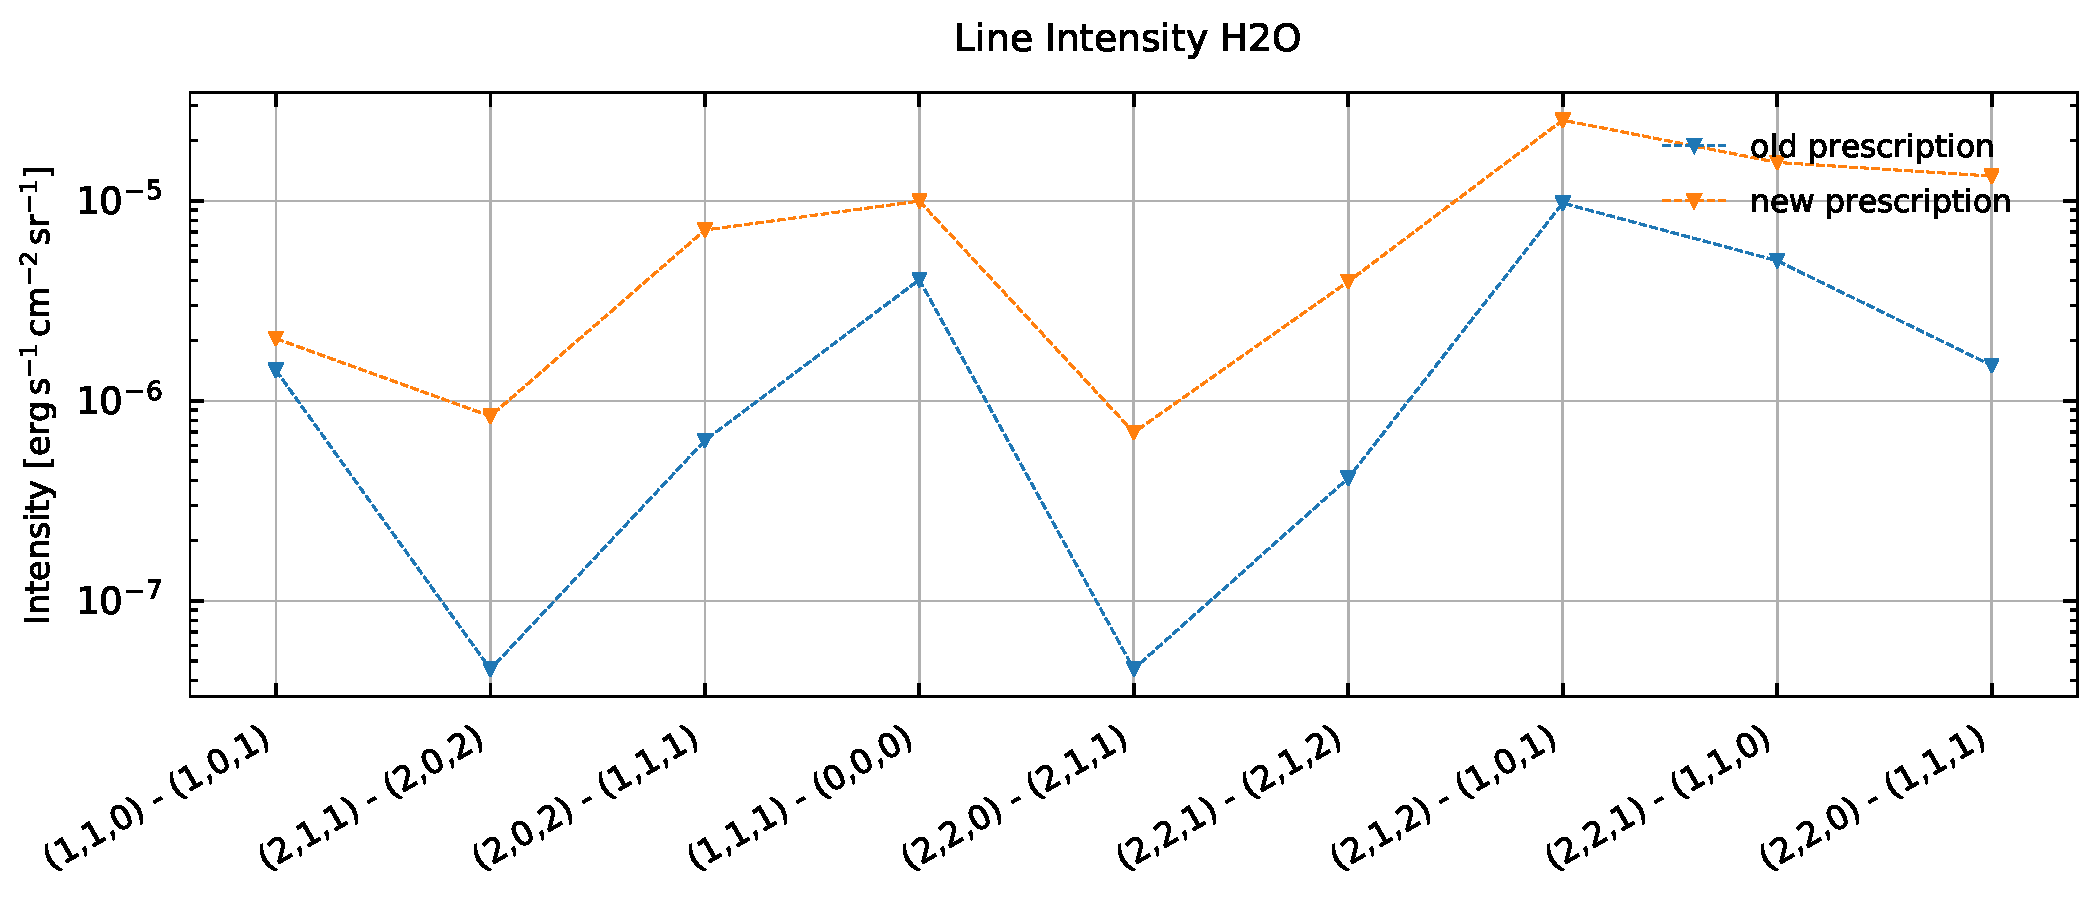
\includegraphics[trim = {0 0 0 1cm},clip,width=0.8\textwidth]{figure/type46/I_comp_H2O.pdf}
    \caption{Diagramme d'excitation du $\mathrm{H}_2\mathrm{O}$}
    \begin{minipage}{\textwidth}
  
    \end{minipage}
    \label{fig:type46:H2O}
\end{figure}



\end{appendices}
